% Rapport scientifique du volet Synthèse
% Compilation : uv run python make_figures.py   puis   latexmk -xelatex rapport.tex
\documentclass[11pt,a4paper]{article}

% --- Langue et polices (XeLaTeX ou LuaLaTeX) -----------------------------------
\usepackage{fontspec}
\usepackage{polyglossia}
\setdefaultlanguage{french}
\setotherlanguage{english}
\usepackage{unicode-math}
\setmathfont{Latin Modern Math}

% --- Mise en page --------------------------------------------------------------
\usepackage[a4paper,margin=2.4cm,headheight=14pt]{geometry}
\usepackage{microtype}
\emergencystretch=2.5em
\usepackage[export]{adjustbox}
\usepackage{graphicx}
\usepackage{booktabs}
\usepackage{array}
\usepackage{multirow}
\usepackage{float}
\usepackage{caption}
\captionsetup{font=small,labelfont=bf,format=hang,labelsep=period}
\usepackage{subcaption}
\usepackage{enumitem}
\setlist{itemsep=2pt,topsep=4pt}
\usepackage{amsmath}
\usepackage{xcolor}
\definecolor{accent}{HTML}{1F5FAD}
\definecolor{ambre}{HTML}{B5650B}
\definecolor{fond}{HTML}{F5F7FA}
\usepackage{tcolorbox}
\tcbuselibrary{skins}
\newtcolorbox{retenir}[1][À retenir]{enhanced,colback=fond,colframe=accent,boxrule=0.6pt,
  arc=2pt,left=7pt,right=7pt,top=5pt,bottom=5pt,title=#1,fonttitle=\bfseries\small,coltitle=white,
  colbacktitle=accent,attach boxed title to top left={xshift=6pt,yshift=-2mm},boxed title style={arc=1pt,boxrule=0pt}}
\newtcolorbox{limite}[1][Limite]{enhanced,colback=white,colframe=ambre,boxrule=0.6pt,
  arc=2pt,left=7pt,right=7pt,top=5pt,bottom=5pt,title=#1,fonttitle=\bfseries\small,coltitle=white,
  colbacktitle=ambre,attach boxed title to top left={xshift=6pt,yshift=-2mm},boxed title style={arc=1pt,boxrule=0pt}}
\usepackage{tikz}
\usetikzlibrary{arrows.meta,positioning,fit,calc}
\usepackage{fancyhdr}
\pagestyle{fancy}
\fancyhf{}
\fancyhead[L]{\small\color{gray}VLM locaux juges de CT synthétiques}
\fancyhead[R]{\small\color{gray}IMT Atlantique · LaTIM}
\fancyfoot[C]{\small\thepage}
\renewcommand{\headrulewidth}{0.4pt}
\usepackage[numbers,sort&compress]{natbib}
\usepackage[hidelinks]{hyperref}
\hypersetup{colorlinks=true,linkcolor=accent,citecolor=accent,urlcolor=accent}
\usepackage[nameinlink,noabbrev]{cleveref}
\crefname{figure}{figure}{figures}
\crefname{table}{tableau}{tableaux}
\crefname{section}{section}{sections}
\crefname{appendix}{annexe}{annexes}
\crefname{equation}{équation}{équations}

% Fichier généré par make_figures.py : ne pas modifier à la main.
\newcommand{\nJudgements}{20\,396}
\newcommand{\nErrors}{2075}
\newcommand{\nModelsVal}{10}
\newcommand{\nModelsTest}{4}
\newcommand{\pctAcceptable}{10}
\newcommand{\pctAcceptableSlices}{35}
\newcommand{\maeEpOne}{249}
\newcommand{\maeEpHundred}{98}
\newcommand{\maeFedsynth}{136}
\newcommand{\bestVal}{Qwen3-VL 30B}
\newcommand{\bestValRho}{0,36 [0,29~; 0,44]}
\newcommand{\bestValIntra}{0,46}
\newcommand{\bestValGen}{0,85}
\newcommand{\bestValAuroc}{0,67}
\newcommand{\bestValGain}{0,42}
\newcommand{\medValRho}{0,27 [0,20~; 0,34]}
\newcommand{\medValGen}{0,81}
\newcommand{\medTestRho}{0,33 [0,26~; 0,41]}
\newcommand{\medTestGen}{0,87}
\newcommand{\medTestAuroc}{0,61}
\newcommand{\medTestGain}{0,31}
\newcommand{\medRgbRho}{$-$0,01 [$-$0,10~; 0,09]}
\newcommand{\medBigStd}{0,5}
\newcommand{\corrMaeSsim}{0,93}
\newcommand{\corrMaeGammaPh}{0,43}
\newcommand{\corrMaeGammaPr}{0,62}
\newcommand{\corrGammaPhPr}{0,33}
\newcommand{\commonValTest}{4}


\newcommand{\tablefile}[1]{{\footnotesize\setlength{\tabcolsep}{4pt}\adjustbox{max width=\textwidth}{\input{tables/#1}}}}
\newcommand{\rhot}{\tilde{\rho}}

\title{\vspace{-1.2cm}%
  {\large\color{gray}UE Projet Commande Entreprise · Sujet A, volet Synthèse}\\[0.6em]
  \textbf{Des VLM locaux peuvent-ils juger la qualité\\ de CT synthétiques\,?}\\[0.3em]
  {\large Banc d'essai sur SynthRAD2023 (IRM\,$\rightarrow$\,CT, cerveau)}}
\author{Pierre Guttierez et l'équipe du sujet A\\[0.2em]
  {\small Encadrant : Vincent Jaouen (IMT Atlantique, LaTIM, UMR 1101)}}
\date{Novembre 2026}

\begin{document}
\maketitle
\thispagestyle{fancy}

\begin{abstract}
\noindent\textbf{Contexte.} En radiothérapie guidée par la seule IRM, un CT synthétique (sCT) remplace le scanner de planification. Juger sa qualité suppose normalement le vrai CT, qui est justement absent en routine. Nous évaluons si des modèles vision--langage (VLM) exécutés localement peuvent servir de juges automatiques, à l'aveugle, de la qualité de sCT.
\textbf{Méthodes.} À partir de SynthRAD2023 (tâche 1, cerveau), nous avons construit un banc d'essai de 270 sCT par partie (27 patients $\times$ 10 générateurs), de qualité volontairement variée : sept checkpoints d'un U-Net 2D entraîné par nos soins et trois modèles pré-entraînés publiés (FedSynthCT-Brain). Chaque sCT est caractérisé par des métriques image (MAE, PSNR, SSIM) et dosimétriques (gamma 2\,\%/2\,mm, écarts de DVH, en photons et en protons). Trois coupes axiales par sCT, soit 810 images par partie, ont été notées de 0 à 100 par \nModelsVal{} VLM locaux (Ollama, sortie JSON imposée, température nulle) selon deux rendus. Le juge est évalué par la corrélation de rang orientée entre sa note et la MAE de la coupe, avec des intervalles de confiance par bootstrap sur les patients, l'AUROC et le gain d'un filtrage.
\textbf{Résultats.} Sur la validation, le meilleur juge est \bestVal{} ($\rhot$~= \bestValRho{}, AUROC = \bestValAuroc{}). Il est significativement meilleur que tous les autres. MedGemma 4B, modèle médical de 4 milliards de paramètres, est deuxième ($\rhot$~= \medValRho{}) et le seul juge confirmé sur le test ($\rhot$~= \medTestRho{}), pour 0,5\,s et 3,4\,Go par image. À l'échelle des générateurs, ces juges classent presque parfaitement les modèles de synthèse ($\rho = 0{,}81$ à $0{,}87$), mais à l'échelle d'une image le signal reste modeste. Plusieurs VLM sont inutilisables (note constante, inversion, boucles de génération), et l'effet du rendu dépend fortement du modèle. Les notes des VLM suivent moins bien la dose que l'apparence de l'image.
\textbf{Conclusion.} Un VLM local, sans entraînement spécifique, fournit un signal de qualité réel mais faible : utile pour comparer des modèles de synthèse ou écarter grossièrement les pires sCT, insuffisant pour accepter ou refuser un sCT individuel en clinique.
\end{abstract}

\vspace{0.4em}
\noindent\textbf{Mots-clés :} CT synthétique, radiothérapie MRI-only, modèle vision--langage, VLM-as-a-judge, évaluation sans vérité terrain, SynthRAD2023.

\tableofcontents
\newpage

% ==================================================================================
\section{Introduction}
\label{sec:intro}

\subsection{Contexte clinique}
En radiothérapie, le scanner (CT) de planification fixe la géométrie du patient et fournit la densité électronique nécessaire au calcul de dose, tandis que l'IRM apporte le contraste des tissus mous pour délinéer la tumeur et les organes à risque. Le flux de travail \emph{MRI-only} cherche à se passer du CT en le synthétisant à partir de l'IRM : on parle de pseudo-CT ou de CT synthétique (sCT)~\cite{bourbonne2021,huijben2024synthrad}. Un sCT doit être à la fois \emph{réaliste} et \emph{dosimétriquement fidèle} : une erreur de densité dans l'os ou les cavités aériques se traduit directement par une erreur de dose.

\subsection{Le verrou : évaluer sans vérité terrain}
Dans un challenge comme SynthRAD2023~\cite{thummerer2023synthrad,huijben2024synthrad}, la qualité d'un sCT se mesure contre le vrai CT du patient (MAE, PSNR, SSIM, gamma, DVH). En routine MRI-only, ce CT n'existe pas : c'est tout l'intérêt de la méthode. Plus généralement, la rareté des annotations de référence et le décalage entre données de développement et données cliniques sont deux obstacles majeurs de l'IA en imagerie~\cite{castro2020causality}. Disposer d'un juge automatique capable d'estimer la qualité d'un sCT \emph{sans} vérité terrain permettrait de contrôler chaque sCT produit, de comparer des modèles de synthèse sur des données non annotées, ou de filtrer des données synthétiques avant un entraînement.

\subsection{Question de recherche}
Le paradigme « grand modèle comme juge » s'est imposé pour évaluer automatiquement du texte~\cite{zheng2023judging}, puis des images. En imagerie médicale, SegAE~\cite{chen2026segae}, un VLM léger entraîné sur des millions de paires synthétiques, prédit la qualité de masques de segmentation 3D avec une corrélation de 0,902 avec le Dice. Notre question, posée par le vade-mecum du projet, est la suivante :

\begin{retenir}[Question de recherche]
Peut-on utiliser un \textbf{VLM local}, sans entraînement spécifique, comme juge automatique de la qualité d'un CT synthétique, \textbf{sans lui montrer la vérité terrain} ? Si oui, \textbf{quel modèle} juge le mieux, et \textbf{à quel coût} ?
\end{retenir}

Le vade-mecum formule aussi une hypothèse à tester : un modèle \emph{médical} (MedGemma) juge-t-il mieux qu'un modèle \emph{généraliste} plus gros ?

\subsection{Contributions}
\begin{enumerate}
  \item Un banc d'essai de 540 sCT (validation et test) de qualité contrôlée et variée, caractérisés par six métriques image et dix métriques dosimétriques (\cref{sec:banc}).
  \item Un protocole de jugement à l'aveugle et reproductible, qui évite toute fuite de la vérité terrain vers le VLM (\cref{sec:methodes}).
  \item Un benchmark de dix VLM locaux, deux rendus, avec des statistiques robustes : intervalles de confiance par patient, comparaisons appariées, corrélation à anatomie égale (\cref{sec:resultats}).
  \item Une analyse critique des causes d'échec des juges et des limites de l'approche (\cref{sec:discussion}).
\end{enumerate}
Ce rapport couvre le volet \emph{synthèse} du sujet A. Le volet \emph{recalage} (champs de déformation pulmonaires) fait l'objet d'un travail séparé.

% ==================================================================================
\section{État de l'art}
\label{sec:etat}

\paragraph{Synthèse de CT.} SynthRAD2023 a fourni 540 paires IRM--CT et CBCT--CT (cerveau et pelvis), et standardisé l'évaluation : métriques image dans le masque du corps et métriques dosimétriques sur des plans recalculés~\cite{thummerer2023synthrad,huijben2024synthrad}. Les meilleures équipes atteignent des MAE de l'ordre de 50 à 60\,HU sur le cerveau. FedSynthCT-Brain~\cite{raggio2025fedsynth} entraîne de façon fédérée plusieurs architectures 2D (dont celles nommées ici Li, Fu et Spadea), diffusées dans l'extension 3D Slicer SlicerModalityConverter~\cite{smc}. Bourbonne, Jaouen \emph{et al.}~\cite{bourbonne2021} ont validé dosimétriquement un pseudo-CT par GAN pour la radiothérapie stéréotaxique cérébrale (gamma, DVH).

\paragraph{Modèles comme juges.} Les LLM utilisés comme évaluateurs atteignent un accord élevé avec des humains sur du texte, mais présentent des biais connus : position, verbosité, complaisance envers la consigne~\cite{zheng2023judging}. Pour les images médicales, SegAE~\cite{chen2026segae} montre qu'un juge \emph{entraîné} pour la tâche peut être très performant.

\paragraph{VLM généralistes et médicaux.} Les VLM ouverts exécutables localement (LLaVA~\cite{liu2023llava}, MiniCPM-V~\cite{yao2024minicpmv}, Qwen3-VL~\cite{qwen3vl}, Gemma) et leurs variantes médicales (MedGemma~\cite{sellergren2025medgemma}) progressent vite, mais leur robustesse aux \emph{artefacts} reste peu étudiée. Or juger une image synthétique revient précisément à juger des artefacts. Le rapport technique de MedGemma 1.5~\cite{medgemma15} recommande un codage du CT en trois fenêtres de HU (une par canal couleur). Nous l'avons testé comme l'un de nos deux rendus.

\paragraph{Positionnement.} La littérature « VLM juge » porte surtout sur des comptes rendus ou des labels 2D. Peu de travaux évaluent des VLM \emph{non entraînés}, \emph{locaux}, sur des \emph{images synthétiques} en les confrontant à des métriques objectives image \emph{et} dosimétriques : c'est la niche de ce travail.

% ==================================================================================
\section{Matériel et méthodes}
\label{sec:methodes}

\begin{figure}[t]
\centering
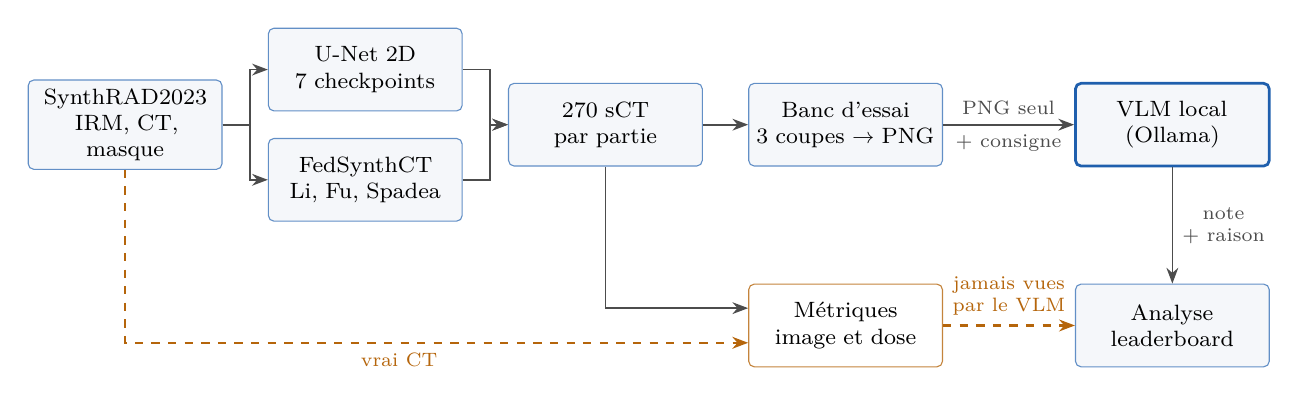
\begin{tikzpicture}[
  box/.style={draw=accent!70,fill=fond,rounded corners=2pt,minimum height=1.05cm,text width=2.25cm,align=center,font=\footnotesize,inner sep=3pt},
  hl/.style={box,draw=accent,line width=1pt},
  arr/.style={-{Stealth[length=2mm]},draw=black!70,line width=0.6pt},
  gt/.style={-{Stealth[length=2mm]},draw=ambre,line width=0.9pt,dashed},
  lab/.style={font=\scriptsize,text=black!70,align=center}]
\node[box] (data) at (0,0) {SynthRAD2023\\IRM, CT, masque};
\node[box] (unet) at (3.05,0.7) {U-Net 2D\\7 checkpoints};
\node[box] (fed)  at (3.05,-0.7) {FedSynthCT\\Li, Fu, Spadea};
\node[box] (sct)  at (6.1,0) {270 sCT\\par partie};
\node[box] (tb)   at (9.15,0) {Banc d'essai\\3 coupes $\to$ PNG};
\node[hl]  (vlm)  at (13.3,0) {VLM local\\(Ollama)};
\node[box] (an)   at (13.3,-2.55) {Analyse\\leaderboard};
\node[box,fill=white,draw=ambre!80] (met) at (9.15,-2.55) {Métriques\\image et dose};
\draw[arr] (data.east) -- ++(0.35,0) |- (unet.west);
\draw[arr] (data.east) -- ++(0.35,0) |- (fed.west);
\draw[arr] (unet.east) -- ++(0.35,0) |- (sct.west);
\draw[arr] (fed.east) -- ++(0.35,0) |- (sct.west);
\draw[arr] (sct) -- (tb);
\draw[arr] (sct.south) |- ($(met.west)+(0,0.22)$);
\draw[arr] (tb) -- node[lab,above]{PNG seul} node[lab,below]{+ consigne} (vlm);
\draw[arr] (vlm) -- node[lab,right]{note\\+ raison} (an);
\draw[gt] (data.south) |- node[lab,pos=0.72,below,text=ambre]{vrai CT} ($(met.west)+(0,-0.22)$);
\draw[gt] (met) -- node[lab,above,text=ambre]{jamais vues\\par le VLM} (an);
\end{tikzpicture}
\caption{Chaîne expérimentale. Le chemin orange (tirets) transporte la vérité terrain : le vrai CT sert uniquement à calculer les métriques de référence, qui vont directement à l'analyse. Le VLM ne reçoit qu'une image et une consigne.}
\label{fig:chaine}
\end{figure}

\subsection{Données}
Nous utilisons la tâche 1 « cerveau » de SynthRAD2023~\cite{thummerer2023synthrad} : 180 patients issus de trois centres (60 par centre, notés A, B, C), chacun avec une IRM T1, un CT et un masque du corps recalés sur une grille commune de 1\,mm. Les patients sont répartis \emph{par patient} et \emph{centre par centre} en apprentissage (126), validation (27) et test (27), avec une graine fixe : toutes les coupes d'un patient restent dans la même partie, et chaque centre est représenté dans chaque partie. La validation sert à tous les réglages (entraînement, rendu, choix du juge). Le test n'est utilisé qu'une fois, à la fin.

\subsection{Génération d'un banc d'essai de qualité variée}
\label{sec:generation}
Pour que la corrélation entre juge et métrique soit informative, il faut un large éventail de qualités. Nous combinons deux sources (\cref{fig:chaine}) :
\begin{itemize}
  \item \textbf{U-Net 2D entraîné par nos soins.} Un \texttt{BasicUNet} de MONAI~\cite{ronneberger2015unet,cardoso2022monai} (canaux 32--32--64--128--256--32) prédit une coupe axiale de CT à partir de la coupe d'IRM correspondante. L'IRM est normalisée par le 99,5\textsuperscript{e} percentile dans le corps, le CT est ramené de $[-1024, 3000]$\,HU vers $[0,1]$. Entraînement : perte L1, Adam ($\eta = 2\cdot10^{-4}$), lots de 16 coupes de $256\times256$, 2\,000 coupes par époque, 100 époques. Nous gardons les checkpoints des époques 1, 2, 5, 10, 20, 50 et 100 : les premiers donnent des sCT flous et faux, les derniers des sCT de bonne qualité.
  \item \textbf{Trois modèles pré-entraînés} de FedSynthCT-Brain~\cite{raggio2025fedsynth,smc}, notés Li, Fu et Spadea, exécutés tels quels dans l'environnement fourni par l'encadrant. Ce sont des réseaux 2D appliqués dans les trois plans puis fusionnés.
\end{itemize}
Chaque partie compte donc $27 \times 10 = 270$ sCT. Les dix générateurs couvrent une MAE moyenne de \maeEpOne{}\,HU (U-Net, époque 1) à \maeEpHundred{}\,HU (U-Net, époque 100) sur le test (\cref{sec:banc}).

\subsection{Métriques de référence}
\label{sec:metriques}
\paragraph{Métriques image.} Comme dans SynthRAD2023, sCT et CT sont d'abord tronqués à l'intervalle $[-1024, 3000]$\,HU, puis comparés dans le masque du corps $M$ :
\begin{equation}
\mathrm{MAE} = \frac{1}{|M|}\sum_{v\in M}\bigl|\,s(v)-c(v)\,\bigr|,\quad
\mathrm{PSNR} = 10\log_{10}\frac{R^2}{\frac{1}{|M|}\sum_{v\in M}\bigl(s(v)-c(v)\bigr)^2},
\label{eq:mae}
\end{equation}
avec $s$ le sCT, $c$ le CT et $R = 4024$\,HU la plage. La SSIM~\cite{wang2004ssim} est calculée sur l'image entière, fond mis à $-1024$\,HU, puis moyennée sur $M$. Ces trois métriques sont calculées sur le \emph{volume entier} et sur la \emph{coupe rendue} : la MAE de la coupe est notre métrique de référence, puisque c'est la seule chose que le VLM voit.

\paragraph{Métriques dosimétriques.} SynthRAD2023 ne fournit ni contours ni plans cliniques. Nous définissons donc pour chaque patient une cible sphérique (PTV) de 15\,mm de rayon, centrée sur les tissus mous de la tête, avec une prescription de 60\,Gy. Un plan est optimisé sur le \emph{vrai} CT avec pyRadPlan~\cite{pyradplan}, portage Python de matRad~\cite{wieser2017matrad} : en photons, IMRT à cinq faisceaux coplanaires (6\,MV, pencil beam SVD) ; en protons, deux faisceaux latéraux opposés (pencil beam). Le plan est normalisé à une dose moyenne de 60\,Gy dans la cible. Il est ensuite recalculé \emph{à l'identique} (mêmes faisceaux, mêmes poids) sur chaque sCT, et les deux distributions de dose sont comparées. L'indice gamma~\cite{low1998gamma}
\begin{equation}
\Gamma(\mathbf{r}) = \min_{\mathbf{r}'}\sqrt{\frac{\lVert\mathbf{r}-\mathbf{r}'\rVert^2}{\Delta d^2}+\frac{\bigl(D_s(\mathbf{r}')-D_c(\mathbf{r})\bigr)^2}{\Delta D^2}}
\end{equation}
est calculé avec PyMedPhys~\cite{pymedphys} (global, $\Delta D = 2\,\%$ du maximum, $\Delta d = 2$\,mm, seuil bas à 10\,\% de la dose maximale). Nous rapportons le taux de points avec $\Gamma \le 1$, l'écart de dose moyen $\Delta D$ là où la dose dépasse 10\,\% du maximum, et les écarts absolus de D98 (couverture) et de D2 (point chaud) de la cible. Les écarts sont exprimés en \% de la prescription.

\subsection{Rendu des images pour le VLM}
\label{sec:rendu}
Pour chaque patient, trois coupes axiales sont prises à 35, 50 et 65\,\% de la hauteur du corps. Ce sont \emph{les mêmes coupes pour les dix sCT du patient}, ce qui permet des comparaisons à anatomie égale. Tout ce qui est hors du masque du corps est mis à l'air ($-1024$\,HU), pour tous les sCT : sinon un VLM pourrait reconnaître un générateur à son fond (bruité pour le U-Net, parfaitement noir pour FedSynthCT) au lieu de juger l'anatomie. La coupe est recadrée sur le corps, puis convertie en image par fenêtrage :
\begin{equation}
I_k(v) = \operatorname{round}\Bigl(255\cdot\operatorname{clip}\Bigl(\frac{h(v)-a_k}{b_k-a_k},0,1\Bigr)\Bigr),
\end{equation}
pour une ou trois fenêtres $[a_k, b_k]$. Deux rendus sont comparés : \textbf{gray}, une fenêtre large $[-1000, 1000]$\,HU en niveaux de gris, $512\times512$ pixels ; \textbf{rgb3}, le codage recommandé pour MedGemma~\cite{medgemma15}, avec R $=[-1024,1024]$, V $=[-135,215]$ et B $=[0,80]$\,HU, en $896\times896$. L'image ne contient aucun texte, aucune légende, rien qui trahisse le générateur ou sa qualité. Chaque partie compte $270 \times 3 = 810$ images par rendu.

\subsection{Juges VLM}
\label{sec:juges}
Dix VLM ouverts, exécutés localement par Ollama~\cite{ollama} sur une RTX~5090 (32\,Go), ont été testés (\cref{tab:modeles}). Chaque image est envoyée avec la même consigne (\emph{prompt}) \texttt{realism\_v1} (\cref{app:prompts}), qui demande d'évaluer le réalisme anatomique et l'absence d'artefacts, et de rendre une note de 0 à 100 avec une courte justification. La sortie est contrainte par un schéma JSON (paramètre \texttt{format} d'Ollama, \texttt{score} entier dans $[0,100]$ et \texttt{reason}), à température nulle avec une graine fixe. Une réponse est plafonnée à 2\,048 jetons. Une réponse coupée à ce plafond, refusée par le serveur ou sans justification est comptée comme un échec. Les modèles sont chargés un par un en mémoire GPU, et la latence et la VRAM de chaque requête sont enregistrées. Au total, \nJudgements{} requêtes ont été journalisées.

\begin{table}[t]
\centering\footnotesize
\caption{VLM évalués. Taille en milliards de paramètres (B), d'après le tag Ollama ; n.\,r. : non relevée.}
\label{tab:modeles}
\begin{tabular}{llrll}
\toprule
Modèle (tag Ollama) & Famille & Taille & Type & Remarque \\
\midrule
\texttt{moondream:latest} & Moondream & 1,8\,B & généraliste & minuscule, test de bout en bout \\
\texttt{llava:7b}, \texttt{llava:13b} & LLaVA~\cite{liu2023llava} & 7 / 13\,B & généraliste & référence répandue \\
\texttt{minicpm-v:8b} & MiniCPM-V~\cite{yao2024minicpmv} & 8\,B & généraliste & bon rapport qualité/taille \\
\texttt{qwen3-vl:8b}, \texttt{qwen3-vl:30b} & Qwen3-VL~\cite{qwen3vl} & 8 / 30\,B & généraliste & 30B : mélange d'experts \\
\texttt{qwen3.8:27b} & Qwen3.8 & 27\,B & généraliste & mode « réflexion » \\
\texttt{gemma4:latest} & Gemma 4 & n.\,r. & généraliste & génération récente \\
\texttt{medgemma:latest} & MedGemma~\cite{sellergren2025medgemma} & 4\,B & \textbf{médical} & images médicales 2D \\
\texttt{medgemma:27b} & MedGemma & 27\,B & \textbf{médical} & version plus grande \\
\bottomrule
\end{tabular}
\end{table}

\subsection{Évaluation des juges}
\label{sec:eval}
\paragraph{Corrélation orientée.} Pour une métrique $m$, nous calculons la corrélation de rang de Spearman~\cite{spearman1904} entre les notes $x$ et les valeurs $y$, orientée pour que $+1$ signifie toujours « le VLM donne les meilleures notes aux meilleurs sCT » :
\begin{equation}
\rhot_m = \sigma_m\,\rho_S(x, y),\qquad \sigma_m = \begin{cases}-1 & \text{si « plus bas = meilleur » (MAE, écarts de dose)}\\ +1 & \text{sinon (PSNR, SSIM, gamma)}\end{cases}
\end{equation}
Un juge qui donne toujours la même note obtient $\rhot = 0$. Le critère principal est $\rhot$ avec la MAE de la coupe, sur les 810 images.

\paragraph{Corrélations complémentaires.} $\rho_\text{intra}$ est la moyenne des $\rhot$ calculés à anatomie égale : pour chaque (patient, coupe), on classe les dix sCT, puis on moyenne sur les 81 groupes. C'est la mesure la plus stricte, car elle ne récompense pas un juge qui réagit seulement au contenu anatomique de la coupe. $\rho_\text{gén}$ est la corrélation entre la note moyenne et la MAE moyenne des dix générateurs : elle mesure la capacité à classer des \emph{modèles} de synthèse. Nous rapportons aussi la corrélation de Pearson.

\paragraph{AUROC.} Une coupe est dite acceptable si sa MAE est inférieure à 100\,HU (35\,\% des coupes). L'AUROC~\cite{hanley1982auc} est la probabilité qu'une coupe acceptable reçoive une meilleure note qu'une coupe non acceptable ; les ex aequo comptent pour moitié. 0,5 correspond au hasard.

\paragraph{Filtrage.} Si l'on ne garde que la moitié des coupes les mieux notées, la MAE moyenne de celles gardées baisse-t-elle ? Nous définissons le gain relatif à un filtrage oracle (qui garderait les vraies meilleures) :
\begin{equation}
G = \frac{\overline{m}_\text{hasard} - \overline{m}_\text{juge}}{\overline{m}_\text{hasard} - \overline{m}_\text{oracle}},
\end{equation}
où $\overline{m}_\text{hasard}$ est la MAE moyenne de toutes les coupes (espérance d'un tri au hasard). $G = 1$ : aussi bien que l'oracle ; $G = 0$ : pas mieux que le hasard. Les ex aequo au seuil se partagent les places restantes au prorata.

\paragraph{Incertitude.} Les intervalles de confiance à 95\,\% sont obtenus par bootstrap percentile~\cite{efron1993bootstrap} ($B = 1\,000$) en tirant les \emph{patients} avec remise, et non les images : les 30 images d'un patient ne sont pas indépendantes. Les comparaisons entre juges ou entre rendus sont \emph{appariées} : mêmes images, mêmes tirages de patients. Une différence est dite significative si son intervalle ne contient pas 0. Aucune correction pour comparaisons multiples n'est appliquée : les intervalles doivent donc être lus comme descriptifs.

\subsection{Protocole et reproductibilité}
Le VLM ne voit jamais le vrai CT, ni les métriques, ni le nom du générateur (\cref{fig:chaine}). Les identifiants d'images ne sont pas transmis au modèle. Les graines (découpage, entraînement, bootstrap, VLM) sont fixées. L'environnement Python est figé par \texttt{uv.lock}, le code est versionné avec git, et chaque requête est journalisée (modèle, consigne, image, note, justification, latence, VRAM, erreur, horodatage). Toute l'analyse est régénérée par deux scripts (\texttt{pipeline/analyze.py}, puis \texttt{report/make\_figures.py}).

% ==================================================================================
\section{Résultats}
\label{sec:resultats}

\subsection{Le banc d'essai couvre une large gamme de qualité}
\label{sec:banc}

\begin{figure}[t]
\centering
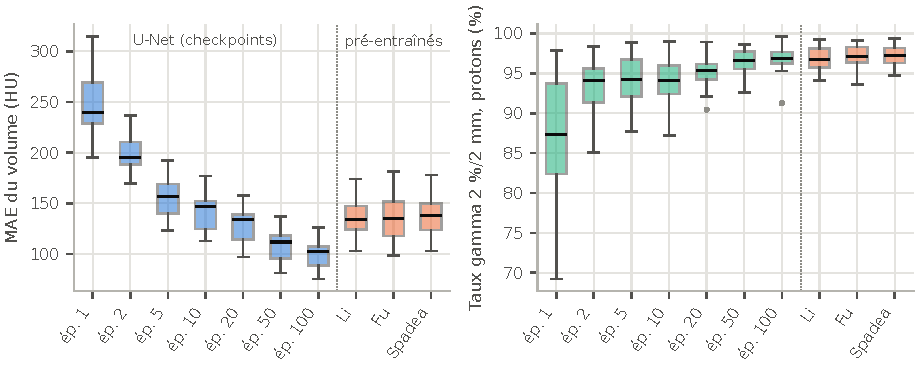
\includegraphics[width=\textwidth]{figures/banc_essai.pdf}
\caption{Qualité des dix générateurs sur les 27 patients de test : (a) MAE du volume ; (b) taux de réussite gamma 2\,\%/2\,mm en protons. En bleu, les checkpoints du U-Net ; en orange, les modèles pré-entraînés.}
\label{fig:banc}
\end{figure}

\begin{table}[t]
\centering
\caption{Qualité moyenne des générateurs sur le test (27 patients). MAE : moyenne $\pm$ écart-type. $\gamma$ : taux de réussite gamma 2\,\%/2\,mm ; $\Delta D$ : écart de dose moyen ; $\Delta D98$ : écart absolu de D98 de la cible ; ph = photons, pr = protons. Les mêmes chiffres sur la validation figurent en \cref{app:val}.}
\label{tab:generateurs}
\tablefile{generateurs_test}
\end{table}

La MAE décroît de façon monotone avec l'entraînement du U-Net : \maeEpOne{}\,HU à l'époque 1, \maeEpHundred{}\,HU à l'époque 100 (\cref{fig:banc,tab:generateurs}). Les trois modèles pré-entraînés se situent autour de \maeFedsynth{}\,HU, entre les époques 10 et 20 du U-Net. Le banc d'essai couvre donc bien la gamme voulue, du très mauvais au bon, mais il ne contient pas de sCT de qualité « état de l'art » (MAE $\approx 50$--60\,HU) : seuls \pctAcceptable{}\,\% des volumes et \pctAcceptableSlices{}\,\% des coupes ont une MAE inférieure à 100\,HU. Les dix générateurs sont presque parfaitement ordonnés de la même façon sur la validation et sur le test (\cref{app:val}).

En dose, la sensibilité dépend fortement de la modalité. En photons, tous les générateurs sauf l'époque 1 dépassent 97\,\% de réussite gamma : la dose photonique est peu sensible aux erreurs de HU. En protons, le taux passe de 87\,\% (époque 1) à 97\,\%. Fait notable, Li, Fu et Spadea ont une MAE \emph{plus élevée} que le U-Net à l'époque 50 ou 100, mais des métriques protons équivalentes ou meilleures ($\gamma_\text{pr} \approx 97\,\%$, $\Delta D_\text{pr} \approx 1{,}3$--1,4\,\%). La MAE ne résume donc pas à elle seule l'utilité dosimétrique.

\paragraph{Biais possible des modèles pré-entraînés.} FedSynthCT-Brain a été entraîné en partie sur le centre C de SynthRAD2023~\cite{raggio2025fedsynth}. Ces modèles ont donc peut-être vu certains de nos patients \texttt{1BC}. Le \cref{tab:centres} montre que le centre C est plus facile \emph{pour tous les générateurs}, y compris le U-Net, qui n'en a vu aucun patient de test. Le rapport des MAE entre les centres C et A est le même pour FedSynthCT (0,73--0,78) et pour le U-Net (0,75--0,80). Nous ne détectons donc pas d'avantage spécifique dû à cette contamination potentielle.

\begin{table}[H]
\centering
\caption{MAE moyenne du volume par centre (validation et test réunis) : le centre C est plus facile pour tous les générateurs, pas seulement pour ceux qui ont pu en voir des patients à l'entraînement.}
\label{tab:centres}
\tablefile{centres}
\end{table}

\subsection{Les métriques de référence ne racontent pas toutes la même histoire}
\label{sec:surrogates}

\begin{figure}[t]
\centering
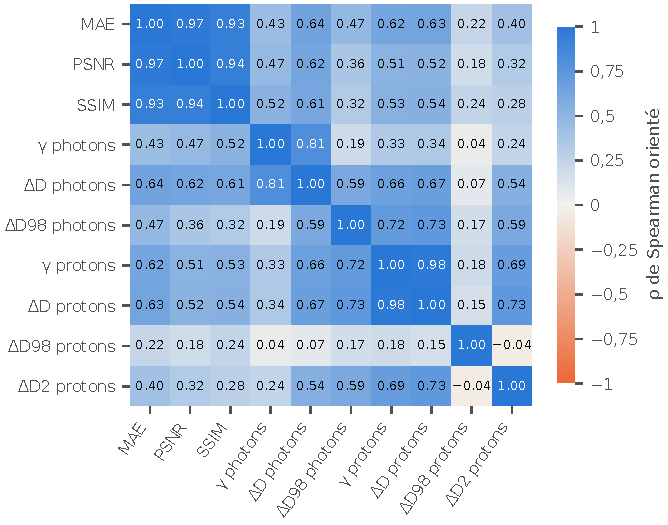
\includegraphics[width=0.78\textwidth]{figures/surrogates.pdf}
\caption{Corrélations de Spearman orientées entre métriques de référence, sur les 540 sCT (validation et test). $+1$ signifie que les deux métriques désignent les mêmes sCT comme meilleurs.}
\label{fig:surrogates}
\end{figure}

Les trois métriques image sont presque redondantes (MAE--SSIM : \corrMaeSsim{}, \cref{fig:surrogates}). Leur lien avec la dose est nettement plus faible : la MAE corrèle à \corrMaeGammaPh{} avec le gamma en photons et à \corrMaeGammaPr{} avec le gamma en protons. Le gamma photons et le gamma protons ne corrèlent qu'à \corrGammaPhPr{} entre eux, et l'écart de D98 en protons est presque indépendant de toutes les autres métriques. Ce constat répond à l'une des questions du vade-mecum : quels \emph{surrogates} reflètent l'utilité clinique ? La MAE est un bon indicateur de ressemblance au CT, mais seulement un indicateur partiel de la fidélité dosimétrique, surtout en photons.

\subsection{Fiabilité technique des juges}
\label{sec:fiabilite}

\begin{figure}[t]
\centering
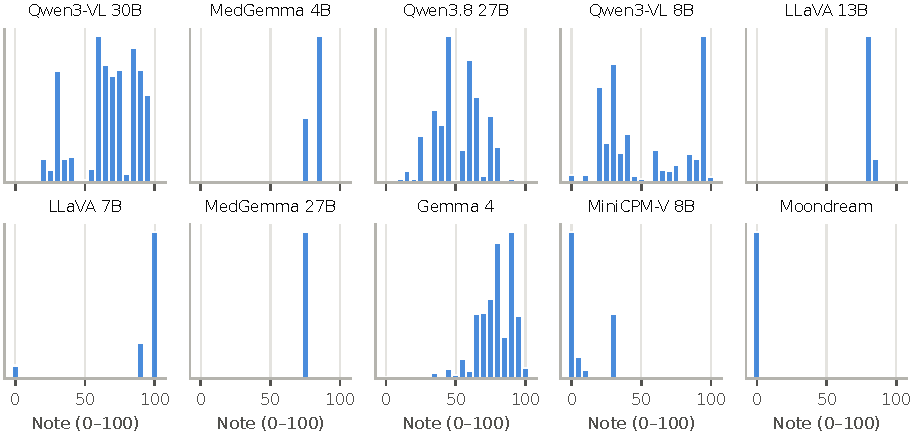
\includegraphics[width=\textwidth]{figures/distributions_val_gray.pdf}
\caption{Distribution des notes de chaque VLM (validation, rendu gray, 810 images, sauf Qwen3-VL 8B : 638 et MiniCPM-V 8B : 56, à cause des erreurs). Plusieurs modèles n'utilisent que quelques valeurs, voire une seule.}
\label{fig:distributions}
\end{figure}

Avant toute corrélation, il faut vérifier que les juges répondent et qu'ils \emph{discriminent}. Trois comportements dégénérés apparaissent (\cref{fig:distributions}) :
\begin{itemize}
  \item \textbf{Note constante.} Moondream donne 0 à toutes les images, avec la justification « \emph{not realistic} ». MedGemma 27B donne 75 à 99,8\,\% des images (écart-type \medBigStd{}), avec des justifications pourtant détaillées et variées. LLaVA 13B donne 80 à 86\,\% des images.
  \item \textbf{Complaisance.} LLaVA 7B donne 100 à 75\,\% des images et affirme l'absence d'artefact dans 92\,\% de ses justifications, y compris pour 93\,\% des sCT de l'époque 1 (\cref{fig:justifications}a). Il recopie souvent la liste d'artefacts de la consigne pour dire qu'aucun n'est présent.
  \item \textbf{Échecs de génération} (\cref{tab:erreurs}). MiniCPM-V 8B ne donne une note valable que pour 23\,\% des images : il part en boucle (arrêt par Ollama ou plafond de jetons atteint) ou rend une justification vide. Qwen3-VL 8B atteint le plafond de 2\,048 jetons sur 17\,\% des images, probablement à cause de son raisonnement interne, qui compte dans ce plafond.
\end{itemize}
Qwen3-VL 30B, Qwen3.8 27B et Gemma 4 utilisent au contraire 20 à 26 valeurs différentes. MedGemma 4B n'en utilise que quatre (65, 75, 85 et 90, dont 85 pour 69\,\% des images), ce qui crée beaucoup d'ex aequo. Cela limite mécaniquement sa corrélation de rang et son intérêt pour le filtrage (\cref{sec:filtrage}).

\begin{table}[H]
\centering
\caption{Images sans note valable, toutes expériences confondues : une image compte une fois par modèle, quel que soit le nombre de requêtes. « Rattrapées » : notées après un nouvel essai. Les autres modèles notent toutes les images du premier coup.}
\label{tab:erreurs}
\tablefile{erreurs}
\end{table}

\subsection{Leaderboard sur la validation}
\label{sec:leaderboard}

\begin{figure}[t]
\centering
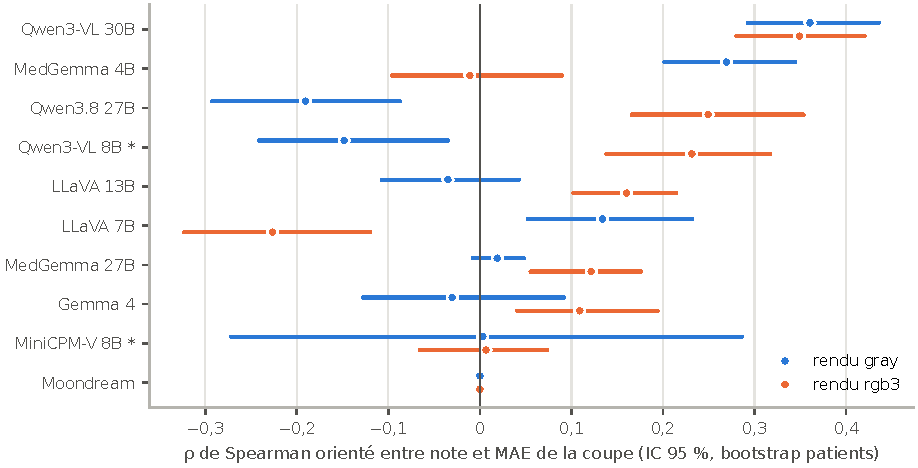
\includegraphics[width=\textwidth]{figures/leaderboard_val.pdf}
\caption{Corrélation orientée entre la note et la MAE de la coupe, pour chaque VLM et chaque rendu (validation, 810 images). Barres : IC 95\,\% par bootstrap sur les patients. * : moins de 90\,\% des images notées sans erreur pour au moins un rendu.}
\label{fig:forest}
\end{figure}

\begin{table}[t]
\centering
\caption{Leaderboard de la validation, rendu gray. Couv. : part des 810 images notées sans erreur ; $\sigma$ : écart-type des notes ; $\rho$ : corrélation orientée avec la MAE de la coupe [IC 95\,\%] ; $\rho_\text{intra}$ : à anatomie égale ; $\rho_\text{gén}$ : au niveau des 10 générateurs ; gain du filtrage à 50\,\% ; latence médiane par image.}
\label{tab:lb-gray}
\tablefile{leaderboard_val_gray}
\end{table}

\begin{table}[t]
\centering
\caption{Leaderboard de la validation, rendu rgb3 (mêmes colonnes que le \cref{tab:lb-gray}).}
\label{tab:lb-rgb3}
\tablefile{leaderboard_val_rgb3}
\end{table}

Avec le rendu gray, \textbf{\bestVal{}} est le meilleur juge (\cref{fig:forest,tab:lb-gray}) : $\rhot$~= \bestValRho{}, $\rho_\text{intra}$~= \bestValIntra{}, AUROC = \bestValAuroc{}, gain de filtrage $G$~= \bestValGain{}. Les comparaisons appariées montrent qu'il est significativement meilleur que \emph{chacun} des neuf autres juges (\cref{tab:pairwise}), y compris MedGemma 4B ($\Delta\rhot = 0{,}09$ [0,02~; 0,16]). MedGemma 4B est deuxième ($\rhot$~= \medValRho{}). Aucun autre juge ne dépasse 0,2 : LLaVA 7B atteint 0,13. Deux juges sont même significativement \emph{inversés} avec ce rendu : Qwen3.8 27B ($-0{,}19$) et Qwen3-VL 8B ($-0{,}15$) donnent en moyenne de meilleures notes aux pires coupes.

\begin{table}[H]
\centering
\caption{Comparaisons appariées avec le meilleur juge (validation, gray) : différence de corrélation orientée et IC 95\,\% bootstrap (mêmes images, mêmes tirages de patients).}
\label{tab:pairwise}
\tablefile{pairwise}
\end{table}

\begin{retenir}
Sur la validation, \bestVal{} est le meilleur juge, significativement. Mais même lui n'explique qu'une petite part du classement des images : $\rhot \approx 0{,}36$, AUROC $\approx 0{,}67$. Le modèle médical MedGemma 4B arrive deuxième, devant des généralistes deux à sept fois plus gros.
\end{retenir}

\subsection{L'effet du rendu dépend du modèle}
\label{sec:rendu-res}

\begin{table}[t]
\centering
\caption{Effet du rendu : différence appariée de corrélation orientée (rgb3 $-$ gray) sur les mêmes coupes, IC 95\,\% bootstrap. « Meilleur rendu » n'est indiqué que si l'intervalle exclut 0.}
\label{tab:delta}
\tablefile{delta_style}
\end{table}

Le rendu change radicalement le comportement de certains juges (\cref{fig:forest,tab:delta}). Le codage rgb3 « retourne » les deux modèles Qwen inversés en gray : $+0{,}44$ pour Qwen3.8 27B, qui passe de $-0{,}19$ à $+0{,}25$, et $+0{,}43$ pour Qwen3-VL 8B. Il améliore aussi LLaVA 13B, Gemma 4 et MedGemma 27B. À l'inverse, il fait perdre tout signal à MedGemma 4B ($-0{,}28$, de 0,27 à $-0{,}01$) et inverse LLaVA 7B ($-0{,}36$). Le meilleur juge, \bestVal{}, est insensible au rendu ($-0{,}01$ [$-0{,}09$~; 0,06]).

Ce résultat est contre-intuitif : MedGemma, le modèle pour lequel le codage rgb3 a été conçu, est le seul juge sérieux qu'il dégrade. Une explication possible, non vérifiée ici, est que la version MedGemma~1 distribuée par Ollama a surtout vu des coupes de CT en niveaux de gris, le codage multi-fenêtres étant associé à MedGemma~1.5 et à son format multi-coupes~\cite{medgemma15}. En pratique, \textbf{le rendu doit être choisi pour chaque modèle}, sur la validation.

\subsection{Le test confirme MedGemma 4B}
\label{sec:test}

\begin{table}[t]
\centering
\caption{Leaderboard du test (rendu gray, 27 patients jamais vus). Seuls les modèles dont le benchmark de test est complet sont listés (voir l'encadré « Limite »).}
\label{tab:lb-test}
\tablefile{leaderboard_test}
\end{table}

\begin{figure}[t]
\centering
\begin{subfigure}[t]{0.49\textwidth}
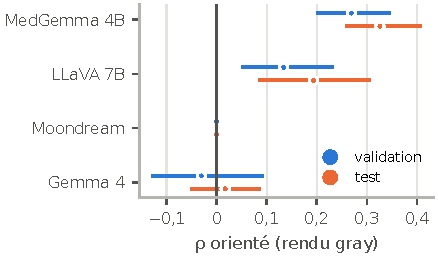
\includegraphics[width=\textwidth]{figures/val_test.pdf}
\caption{Validation et test (rendu gray), pour les modèles évalués sur les deux.}
\label{fig:valtest}
\end{subfigure}\hfill
\begin{subfigure}[t]{0.49\textwidth}
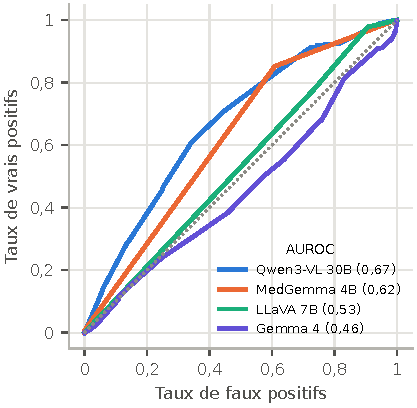
\includegraphics[width=\textwidth]{figures/roc.pdf}
\caption{Courbes ROC (validation, gray), coupe acceptable si MAE $< 100$\,HU.}
\label{fig:roc}
\end{subfigure}
\caption{Stabilité et pouvoir de discrimination des juges.}
\end{figure}

Sur le test, MedGemma 4B atteint $\rhot$~= \medTestRho{}, $\rho_\text{gén}$~= \medTestGen{}, AUROC = \medTestAuroc{} et un gain de filtrage $G$~= \medTestGain{} (\cref{tab:lb-test}). Les \commonValTest{} modèles évalués sur les deux parties gardent le même ordre et des corrélations compatibles (\cref{fig:valtest}) : le classement obtenu sur la validation se généralise à des patients nouveaux.

\begin{limite}[Limite : benchmark de test incomplet]
Le benchmark de test a été interrompu après les quatre premiers modèles (Moondream, MedGemma 4B, LLaVA 7B, Gemma 4), et Qwen3-VL 8B n'y a noté que 26 images. \textbf{Le meilleur juge de la validation, \bestVal{}, n'a donc pas été évalué sur le test}, ni Qwen3.8 27B, LLaVA 13B, MedGemma 27B et MiniCPM-V 8B. Sa première place repose sur la validation seule, où il a aussi été sélectionné : elle peut être légèrement optimiste (effet du gagnant). Compléter le test (environ 4\,h de calcul d'après les latences mesurées sur la validation) est la première chose à faire avant toute conclusion définitive (\cref{sec:perspectives}).
\end{limite}

\subsection{Un juge de modèles plutôt qu'un juge d'images}
\label{sec:generateurs}

\begin{figure}[t]
\centering
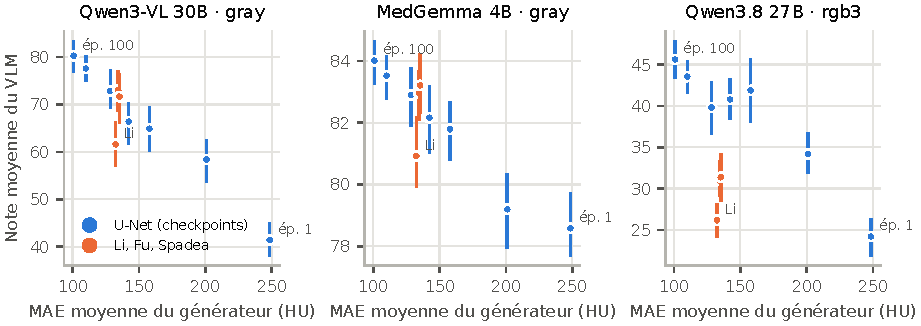
\includegraphics[width=\textwidth]{figures/scores_generateurs.pdf}
\caption{Note moyenne de trois juges pour chacun des dix générateurs, en fonction de la MAE moyenne du générateur (validation ; barres : IC 95\,\% bootstrap sur les patients).}
\label{fig:generateurs}
\end{figure}

À l'échelle d'une image, les corrélations restent modestes. Mais en moyennant les notes par générateur, les bons juges classent presque parfaitement les dix modèles de synthèse : $\rho_\text{gén}$~= \bestValGen{} pour \bestVal{}, \medValGen{} pour MedGemma 4B sur la validation et \medTestGen{} sur le test (\cref{tab:lb-gray,tab:lb-test,fig:generateurs}). Le bruit d'un jugement individuel se moyenne sur les 81 images d'un générateur. Les modèles pré-entraînés Li, Fu et Spadea reçoivent des notes plus basses que le U-Net à MAE comparable, surtout chez Qwen3.8 27B : les juges réagissent à une différence de \emph{style} d'image, pas seulement d'erreur.

La corrélation à anatomie égale est \emph{plus élevée} que la corrélation globale pour les meilleurs juges (0,46 contre 0,36 pour \bestVal{}, 0,38 contre 0,27 pour MedGemma 4B, en gray). Une partie du bruit vient donc du contenu de la coupe : certaines régions anatomiques ont une MAE élevée quel que soit le générateur, et le VLM ne le « sait » pas. Le \cref{tab:position} le confirme. MedGemma 4B est presque aveugle sur la coupe basse, où l'on trouve la base du crâne et les sinus ($\rhot = 0{,}11$), mais nettement meilleur sur la coupe haute (0,42). \bestVal{} est plus régulier.

\begin{table}[H]
\centering
\caption{Corrélation orientée selon la position de la coupe (validation, gray, 270 images par position).}
\label{tab:position}
\tablefile{position}
\end{table}

\subsection{Filtrage}
\label{sec:filtrage}

\begin{figure}[t]
\centering
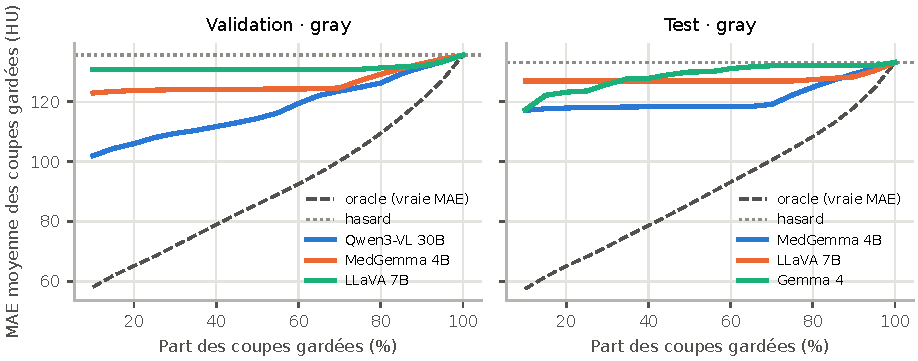
\includegraphics[width=\textwidth]{figures/filtrage.pdf}
\caption{Filtrage par le juge : MAE moyenne des coupes gardées selon la part gardée (les mieux notées d'abord), comparée à un filtrage oracle (vraie MAE) et au hasard.}
\label{fig:filtrage}
\end{figure}

Garder la moitié des coupes les mieux notées par \bestVal{} fait passer la MAE moyenne de 136 à 114\,HU sur la validation, soit $G$~= \bestValGain{} du gain d'un oracle (\cref{fig:filtrage}). Avec MedGemma 4B, le gain est de 0,23 sur la validation et de 0,31 sur le test. La courbe de MedGemma 4B est plate tant que l'on garde moins de 60\,\% des coupes : ses quatre seules valeurs de note ne permettent pas de trier finement le haut du classement. Le filtrage est donc réel mais grossier : il écarte les sCT les plus mauvais, il ne sélectionne pas les meilleurs. Le protocole du vade-mecum prévoit ensuite de réentraîner un modèle sur les données filtrées : cette étape n'a pas été réalisée (\cref{sec:limites}).

\subsection{Les juges suivent l'apparence plus que la dose}
\label{sec:dose}

\begin{table}[H]
\centering
\caption{Corrélation orientée entre la note du VLM et les métriques du volume, image et dose (val = validation).}
\label{tab:dosecorr}
\tablefile{dose_corr}
\end{table}

Les notes corrèlent mieux avec les métriques image du volume (MAE, SSIM : 0,21 à 0,42) qu'avec les métriques de dose (\cref{tab:dosecorr}). Avec le gamma protons, la métrique de dose la plus discriminante, on obtient 0,28 pour \bestVal{} et 0,15 à 0,17 pour MedGemma 4B. Avec l'écart de D98, toutes les valeurs sont inférieures ou égales à 0,12. C'est attendu : le VLM juge le réalisme visuel d'une coupe, alors que la dose dépend de la densité intégrée le long des faisceaux, en 3D. Un juge visuel ne peut pas remplacer une vérification dosimétrique.

\subsection{Ce que disent les justifications}
\label{sec:justif}

\begin{figure}[t]
\centering
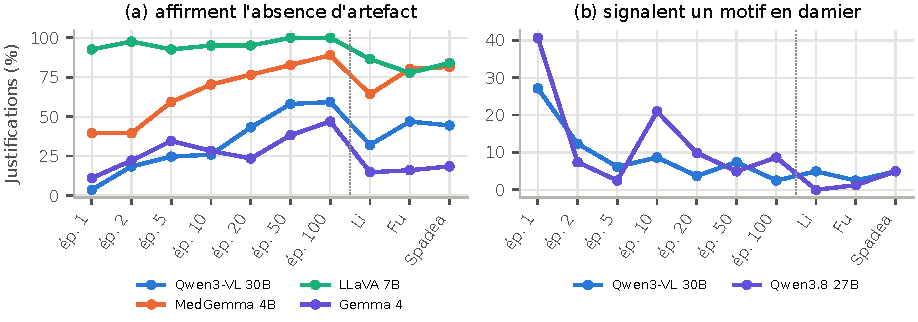
\includegraphics[width=\textwidth]{figures/justifications.pdf}
\caption{Analyse des justifications (validation, gray) : part de celles qui (a) affirment l'absence d'artefact, (b) signalent un motif en damier, par générateur.}
\label{fig:justifications}
\end{figure}

Les justifications permettent de comprendre \emph{pourquoi} un juge réussit ou échoue (\cref{fig:justifications}). Chez \bestVal{} et MedGemma 4B, l'affirmation « pas d'artefact » devient de plus en plus fréquente à mesure que le U-Net s'améliore : de 4 à 59\,\% pour Qwen3-VL 30B, de 40 à 89\,\% pour MedGemma 4B. Leurs justifications sont donc cohérentes avec leurs notes. LLaVA 7B l'affirme presque toujours, ce qui confirme sa complaisance. Surtout, \bestVal{} et Qwen3.8 27B signalent un \emph{motif en damier} sur 27 et 41\,\% des sCT de l'époque 1. C'est un artefact typique des couches de sur-échantillonnage d'un réseau peu entraîné, et donc un vrai défaut détecté.

Le \cref{tab:exemple} compare les justifications de trois juges pour une même coupe d'un patient de validation. Le juge le plus performant décrit des défauts précis, le juge médical répond de façon presque identique aux trois images, et le juge complaisant recopie la consigne.

\begin{table}[H]
\centering\footnotesize
\caption{Justifications (tronquées) de trois juges pour la même coupe (65\,\% de la hauteur) du patient de validation 1BC027, rendu gray. Exemple choisi pour illustrer les trois comportements, et non tiré au hasard.}
\label{tab:exemple}
\begin{tabular}{>{\raggedright\arraybackslash}p{2.6cm}>{\raggedright\arraybackslash}p{2.1cm}>{\raggedright\arraybackslash}p{9.9cm}}
\toprule
sCT (MAE) & Note & Justification \\
\midrule
\multicolumn{3}{l}{\textbf{Qwen3-VL 30B}}\\
Ép. 1 (133\,HU) & 30 & \textit{\foreignlanguage{english}{The image contains a prominent checkerboard pattern (a common AI-generated artifact) and lacks the nuanced contrast between bone, soft tissue, and air\ldots}} \\
Ép. 100 (49\,HU) & 95 & \textit{\foreignlanguage{english}{The image depicts a plausible axial brain CT slice with sharp boundaries between the skull (bright white) and soft tissue (gray), realistic contrast\ldots{} and no visible artifacts\ldots}} \\
Li (63\,HU) & 75 & \textit{\foreignlanguage{english}{\ldots{} However, the brain parenchyma lacks the natural textural variation and subtle\ldots}} \\
\midrule
\multicolumn{3}{l}{\textbf{MedGemma 4B}}\\
Ép. 1 / 100 / Li & 85 / 85 / 85 & \textit{\foreignlanguage{english}{The image appears to be a CT scan of the head. The anatomy is generally plausible, with clear boundaries between bone, soft tissue, and air. There are no obvious artifacts\ldots}} \\
\midrule
\multicolumn{3}{l}{\textbf{LLaVA 7B}}\\
Ép. 1 / 100 / Li & 90 / 100 / 90 & \textit{\foreignlanguage{english}{\ldots{} no apparent artifacts such as blur, unusual noise, checkerboard patterns, or missing\ldots}} (liste recopiée de la consigne) \\
\bottomrule
\end{tabular}
\end{table}

\IfFileExists{figures/exemples.pdf}{%
\begin{figure}[t]
\centering
\includegraphics[width=\textwidth]{figures/exemples.pdf}
\caption{Exemples d'images soumises aux juges : une même coupe du vrai CT et de cinq sCT, avec la MAE de la coupe et les notes de deux juges (test, rendu gray). Le vrai CT n'est jamais montré aux VLM : il ne figure ici que pour la comparaison.}
\label{fig:exemples}
\end{figure}}{}

\subsection{Coût}
\label{sec:cout}

\begin{figure}[t]
\centering
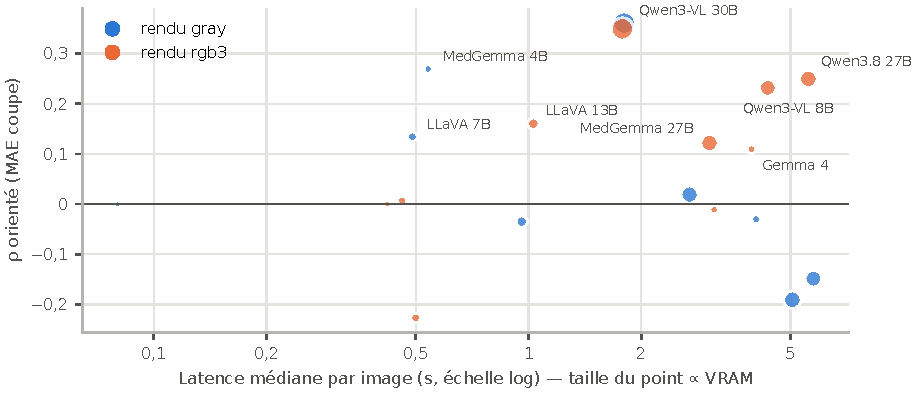
\includegraphics[width=\textwidth]{figures/cout.pdf}
\caption{Compromis performance--coût : corrélation orientée en fonction de la latence médiane par image (validation). La taille du point est proportionnelle à la VRAM utilisée.}
\label{fig:cout}
\end{figure}

MedGemma 4B est de loin le juge le plus économe parmi ceux qui ont un signal : 0,5\,s par image et 3,4\,Go de VRAM (\cref{fig:cout}). \bestVal{} demande 26,9\,Go, presque toute la carte, mais reste rapide (1,8\,s) grâce à son architecture en mélange d'experts : seule une fraction de ses paramètres est active à chaque jeton. Les modèles denses de 27\,B coûtent 2,7 à 5,6\,s par image, pour un signal nul (MedGemma 27B) ou qui dépend entièrement du rendu (Qwen3.8 27B). Noter les 810 images d'une partie prend donc 7\,min avec MedGemma 4B, 27\,min avec \bestVal{} et plus d'une heure avec Qwen3.8 27B. Le rendu compte aussi : en rgb3 ($896\times896$ pixels), la latence de MedGemma 4B passe de 0,5 à 3,1\,s.

% ==================================================================================
\section{Discussion}
\label{sec:discussion}

\subsection{Réponse à la question de recherche}
\textbf{Oui, partiellement.} Sans aucun entraînement spécifique et sans voir le vrai CT, deux VLM locaux sur dix produisent un signal de qualité significatif et stable : \bestVal{} et MedGemma 4B. Ce signal suffit à \emph{classer des modèles de synthèse} ($\rho_\text{gén} \ge 0{,}8$) et à écarter grossièrement les pires sCT (gain de filtrage de 0,2 à 0,4). Il est en revanche trop faible pour juger un sCT \emph{individuel} : avec une AUROC de 0,6--0,7, un tel juge accepterait ou refuserait à tort une proportion importante de sCT. Il ne reflète que partiellement la fidélité dosimétrique. Nous sommes loin des 0,902 de SegAE~\cite{chen2026segae}, et de sa vitesse : 0,06\,s par masque 3D, contre 1,8\,s par coupe 2D pour \bestVal{}, soit plus de 5\,s pour les trois coupes d'un sCT. La comparaison n'est cependant pas directe : SegAE est un juge \emph{entraîné} sur plus de quatre millions d'exemples pour une tâche précise (des masques), alors que nos VLM sont utilisés tels quels, en zéro-coup.

\subsection{Modèle médical ou généraliste plus gros ?}
L'hypothèse du vade-mecum reçoit une réponse nuancée. Le petit modèle médical MedGemma 4B fait au moins aussi bien que tous les généralistes de 7 à 27\,B, chacun pris dans son meilleur rendu, et reste le seul juge confirmé sur le test, pour un coût minimal. Mais il est battu par le plus gros généraliste, Qwen3-VL 30B. Et la version médicale de 27\,B s'effondre sur une note constante. Ni la spécialisation, ni la taille ne garantissent un bon juge : en gray, LLaVA 13B fait moins bien que LLaVA 7B, et Qwen3.8 27B est inversé. Ce qui distingue \bestVal{}, c'est sa capacité à \emph{utiliser toute l'échelle de notes} et à \emph{décrire des défauts précis} plutôt qu'à paraphraser la consigne. MedGemma 4B, lui, n'utilise que quatre notes, mais les attribue dans le bon ordre.

\subsection{Pourquoi les juges échouent}
Nous identifions quatre mécanismes, visibles directement dans les données :
\begin{enumerate}
  \item \textbf{L'ancrage sur une note par défaut} : 75 pour MedGemma 27B, 80 pour LLaVA 13B, 0 pour Moondream. La consigne donne les bornes 0 et 100 sans graduation intermédiaire, et certains modèles se replient sur une valeur « prudente ».
  \item \textbf{La complaisance envers la consigne} (biais de prompt signalé par le vade-mecum) : LLaVA 7B reprend la liste d'artefacts de la consigne pour affirmer leur absence et donne 100 dans 75\,\% des cas.
  \item \textbf{La sensibilité à la représentation de l'image}, qui peut inverser le signal d'un modèle (\cref{sec:rendu-res}).
  \item \textbf{Les échecs de génération} sous contrainte JSON : boucles de MiniCPM-V, raisonnement trop long de Qwen3-VL 8B. Ils réduisent la couverture et peuvent biaiser l'échantillon noté.
\end{enumerate}
Enfin, un VLM ne voit qu'une coupe 2D sans référence. Il ne peut pas savoir qu'un os est un peu trop peu dense, ce qui suffit pourtant à créer une erreur de dose en protons. Il juge le \emph{réalisme}, qui n'est qu'une condition nécessaire de la \emph{justesse}.

\subsection{Limites}
\label{sec:limites}
\begin{itemize}
  \item \textbf{Test incomplet} : le meilleur juge de la validation n'a pas été évalué sur le test (\cref{sec:test}).
  \item \textbf{Une seule consigne} (\texttt{realism\_v1}) a été évaluée. Deux variantes ont été préparées (barème explicite, recherche de défauts, \cref{app:prompts}) mais non testées. Le réglage a porté uniquement sur le rendu.
  \item \textbf{Comparaisons multiples} : 20 configurations (modèle, rendu) ont été comparées sur la validation sans correction. Les intervalles sont descriptifs, et le meilleur juge peut bénéficier d'un effet du gagnant.
  \item \textbf{Taille de l'échantillon} : 27 patients par partie. Les intervalles de confiance restent larges : $\pm 0{,}07$ pour le meilleur juge, $\pm 0{,}09$ en moyenne.
  \item \textbf{Échecs non aléatoires} : en rgb3, Qwen3-VL 8B échoue sur 2\,\% des sCT de l'époque 1 mais sur 22\,\% de ceux de l'époque 100. Les bonnes images sont donc sous-représentées dans sa corrélation.
  \item \textbf{Banc d'essai} : pas de sCT de qualité état de l'art (MAE $< 70$\,HU en moyenne), pas de défauts « cliniques » ciblés (os manquant, sinus rempli). Les juges n'ont donc pas été testés sur la distinction la plus utile en pratique, entre « bon » et « très bon ».
  \item \textbf{Métrique de référence 2D} : la MAE d'une coupe est une cible bruitée (sensible au contenu anatomique), qui explique une partie des corrélations modestes.
  \item \textbf{Dose} : la cible sphérique, la prescription et les faisceaux sont synthétiques. Ils mesurent l'effet des erreurs du sCT sur un plan réaliste, pas sur le plan réel du patient.
  \item \textbf{Boucle de filtrage incomplète} : le gain est mesuré sur la MAE des sCT gardés, sans réentraînement d'un modèle sur les données filtrées.
  \item \textbf{Versions des modèles} : les tags Ollama (par ex. \texttt{latest}) évoluent. Il faudra enregistrer leurs empreintes (\texttt{ollama list}) pour une reproductibilité stricte.
\end{itemize}

\subsection{Perspectives}
\label{sec:perspectives}
\begin{enumerate}
  \item \textbf{Compléter le test} avec les six modèles manquants, au moins \bestVal{}, Qwen3.8 27B (en rgb3) et Qwen3-VL 8B (en rgb3), chacun avec le rendu choisi sur la validation : \texttt{bash run\_all.sh test gray}, puis le même en rgb3 pour les modèles concernés.
  \item \textbf{Rattraper les échecs techniques.} Le pipeline retente désormais une image en échec, jusqu'à deux fois : rappel du format JSON attendu, puis un peu d'aléa et une pénalité de répétition. Les modèles qui réfléchissent reçoivent un plafond de 8\,192 jetons. L'essai qui a donné la note est enregistré. Relancer la validation pour Qwen3-VL 8B et MiniCPM-V 8B corrigerait leur couverture, et donc le biais signalé plus haut.
  \item \textbf{Améliorer la consigne} : barème explicite (\texttt{brain\_rubric\_v1}), recherche de défauts (\texttt{defects\_v1}), notation par paires (« laquelle des deux coupes est la plus réaliste ? »), qui évite le problème d'échelle.
  \item \textbf{Donner plus de contexte} : plusieurs coupes par sCT, ou l'IRM source à côté du sCT, puisque l'IRM est disponible en clinique, contrairement au CT.
  \item \textbf{Combiner les juges} (moyenne des rangs de \bestVal{} et MedGemma 4B), ou calibrer leurs notes sur un petit ensemble annoté.
  \item \textbf{Adapter un juge} : un affinage léger de MedGemma 4B sur des paires (sCT, MAE), dans l'esprit de SegAE, est la piste la plus prometteuse pour franchir le plafond du zéro-coup.
  \item \textbf{Étendre} à la tâche CBCT\,$\rightarrow$\,CT de SynthRAD2023, et réaliser la boucle de filtrage complète avec réentraînement.
\end{enumerate}

% ==================================================================================
\section{Conclusion}
Nous avons construit un banc d'essai contrôlé de CT synthétiques et évalué à l'aveugle dix VLM locaux comme juges de leur qualité. Deux modèles se dégagent : \bestVal{}, le plus performant ($\rhot = 0{,}36$), et MedGemma 4B, un peu moins bon mais confirmé sur le test et huit fois moins gourmand en mémoire. Leur signal est réel mais faible à l'échelle d'une image, fort à l'échelle d'un modèle de synthèse, et plus lié à l'apparence qu'à la dose. Les VLM locaux sont donc aujourd'hui des outils d'aide utiles pour comparer des méthodes de synthèse ou trier grossièrement des données, pas des substituts à une vérification dosimétrique. Le choix du rendu et la formulation de la consigne pèsent autant que le choix du modèle, et doivent être réglés sur une validation distincte, comme nous l'avons fait.

\bibliographystyle{unsrtnat}
\bibliography{references}

% ==================================================================================
\appendix
\section{Correspondance avec le vade-mecum}
\label{app:vademecum}

\begin{table}[H]
\centering\footnotesize
\caption{Ce que demande le vade-mecum du projet (sujet A, synthèse) et où ce rapport y répond.}
\begin{tabular}{>{\raggedright\arraybackslash}p{5.6cm}>{\raggedright\arraybackslash}p{1.5cm}>{\raggedright\arraybackslash}p{7.7cm}}
\toprule
Demande du vade-mecum & Statut & Où, et comment \\
\midrule
Question de recherche : un VLM local peut-il juger, lequel, à quel coût ? & traité & \cref{sec:intro,sec:resultats}, discussion \\
Banc d'essai de qualité variée (checkpoints, cas d'échec) & traité & 7 checkpoints + 3 modèles publiés, \cref{sec:banc} ; pas de cas d'échec ciblés \\
Métriques image MAE, PSNR, SSIM & traité & \cref{sec:metriques}, \cref{tab:generateurs} \\
Métriques aval : gamma 2\,\%/2\,mm, écarts de DVH, $D_\text{max}$, $D_\text{mean}$ & traité & photons et protons, plan synthétique ; D2 pour $D_\text{max}$, dose moyenne au corps, \cref{sec:metriques,sec:surrogates} \\
Rendu lisible, plusieurs styles & traité & gray et rgb3, \cref{sec:rendu,sec:rendu-res} \\
Sortie structurée obligatoire (\texttt{format}) & traité & schéma JSON, \cref{sec:juges} \\
Spearman, Pearson, AUROC, temps, mémoire & traité & \cref{sec:eval}, \cref{tab:lb-gray,tab:lb-rgb3,tab:lb-test} \\
Leaderboard et figures & traité & \cref{fig:forest}, \cref{tab:lb-gray,tab:lb-test} \\
Hypothèse « médical vs généraliste plus gros » & traité & \cref{sec:discussion} \\
Juger le réalisme \emph{et} la pertinence clinique & partiel & réalisme seulement ; lien avec la dose en \cref{sec:dose} \\
Filtrage comparé à l'oracle et au hasard & partiel & \cref{sec:filtrage} ; sans réentraînement \\
Ne jamais montrer la vérité terrain & traité & \cref{fig:chaine}, \cref{sec:rendu} \\
Reproductibilité (graines, versions, journal, git) & traité & \cref{sec:methodes} ; empreintes des modèles à ajouter \\
Analyse critique (artefacts, biais) & traité & \cref{sec:fiabilite,sec:justif}, discussion \\
AUROC avec un seuil « acceptable » & traité & MAE de la coupe $< 100$\,HU, \cref{sec:eval} \\
Éviter le biais de prompt, tester des formulations neutres & partiel & une seule consigne évaluée ; biais observés en \cref{sec:fiabilite} \\
Confidentialité : aucune donnée hors de la station & traité & VLM locaux (Ollama), aucune API externe \\
Livrables : figures, rapport, présentation & traité & ce rapport et le diaporama de restitution \\
Juge transversal (synthèse, recalage, segmentation) & non traité & volet recalage et sujet B séparés \\
CBCT\,$\rightarrow$\,CT & non traité & perspective \\
\bottomrule
\end{tabular}
\end{table}

\paragraph{Réponses aux questions de brainstorming (phase 1).}
\begin{enumerate}
  \item \emph{Quelle métrique sert d'étalon ?} Pour la synthèse, le vrai CT existe dans SynthRAD2023 : la MAE dans le corps est l'étalon de ressemblance, et le gamma (surtout en protons) celui de l'utilité dosimétrique. Ils ne sont corrélés qu'à 0,43--0,62 (\cref{sec:surrogates}).
  \item \emph{Quels artefacts un VLM doit-il reconnaître ?} Flou, motif en damier dû au sur-échantillonnage, densité osseuse fausse, cavités aériques mal rendues, textures de tissus non naturelles. Le meilleur juge en signale certains (\cref{sec:justif}).
  \item \emph{Comment rendre la prédiction lisible sans montrer la vérité ?} Fenêtrage, recadrage sur le corps, fond masqué, aucun texte. Le meilleur codage dépend du modèle (\cref{sec:rendu-res}).
  \item \emph{Quels surrogates sont corrélés à l'utilité clinique ?} Les métriques image sont redondantes entre elles, mais seulement partiellement liées à la dose. Gamma et DVH ne mesurent pas la même chose (\cref{fig:surrogates}).
  \item \emph{Quels VLM tiennent sur la carte, à quel coût ?} Tous les dix tiennent sur 32\,Go, de 1 à 27\,Go de VRAM et de 0,1 à 6\,s par image (\cref{fig:cout}).
\end{enumerate}

\section{Consignes envoyées aux VLM}
\label{app:prompts}
Consigne utilisée pour toutes les expériences (\texttt{realism\_v1}) :
\begin{quote}\small\ttfamily\raggedright
This image is an axial slice of a CT scan. It may have been generated by an AI model from an MRI or a CBCT. Assess how anatomically realistic it is: plausible anatomy, sharp boundaries between tissues, realistic contrast between bone, soft tissue and air, and absence of artifacts (blur, unusual noise, checkerboard patterns, missing or distorted structures). Give a score from 0 (clearly unrealistic) to 100 (indistinguishable from a real CT), and a short justification.
\end{quote}
Schéma de sortie imposé : \texttt{\{"score": entier de 0 à 100, "reason": texte\}}. Paramètres : température 0, graine 42, au plus 2\,048 jetons. Deux variantes prêtes mais non évaluées figurent dans \texttt{pipeline/config.py} : \texttt{brain\_rubric\_v1} (barème par tranches de 20 points, points à vérifier sur un crâne) et \texttt{defects\_v1} (partir de 100 et retirer des points par défaut trouvé).

\section{Résultats complémentaires sur la validation}
\label{app:val}
\begin{table}[H]
\centering
\caption{Qualité moyenne des générateurs sur la validation (mêmes colonnes que le \cref{tab:generateurs}).}
\tablefile{generateurs_val}
\end{table}

\begin{figure}[H]
\centering
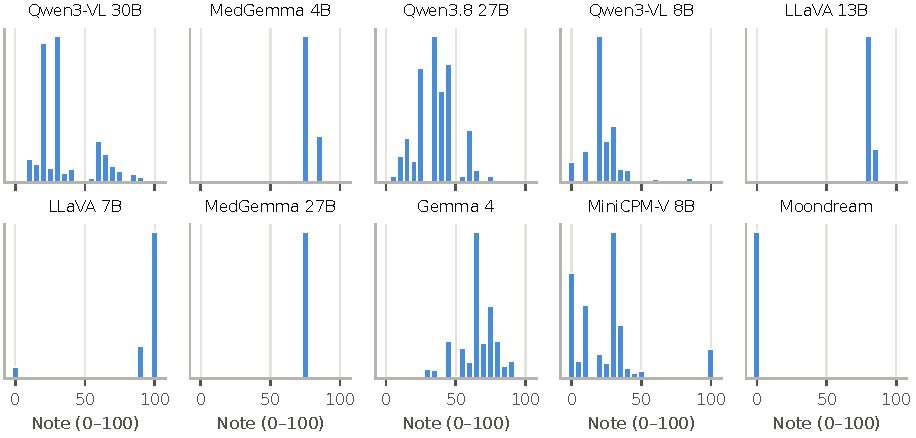
\includegraphics[width=\textwidth]{figures/distributions_val_rgb3.pdf}
\caption{Distribution des notes de chaque VLM, validation, rendu rgb3.}
\end{figure}

\section{Reproduire ce rapport}
\label{app:repro}
Toutes les commandes se lancent depuis le dossier \texttt{Synthesis/} du dépôt ; le détail est dans le mode d'emploi du volet Synthèse.
\begin{enumerate}
  \item Sur la station : produire les sCT, le banc d'essai, les notes et l'analyse, par exemple \texttt{DOSE=1 bash run\_all.sh val} puis \texttt{DOSE=1 bash run\_all.sh test gray}.
  \item Rapatrier \texttt{results/} sur le PC (\texttt{scp -r}).
  \item Dans \texttt{report/} : \texttt{uv run python make\_figures.py}, puis \texttt{latexmk -xelatex rapport.tex}.
  \item Facultatif, sur la station : \texttt{uv run python make\_example\_figure.py} produit une figure d'exemples d'images, incluse automatiquement si elle est présente.
\end{enumerate}
Les figures, tableaux et chiffres du texte sont régénérés à partir des fichiers de résultats. Si les résultats changent, relire la discussion, qui reste rédigée à la main.

\end{document}
